
\begin{frame}
		\frametitle{Serial Sort}
		\begin{figure}
				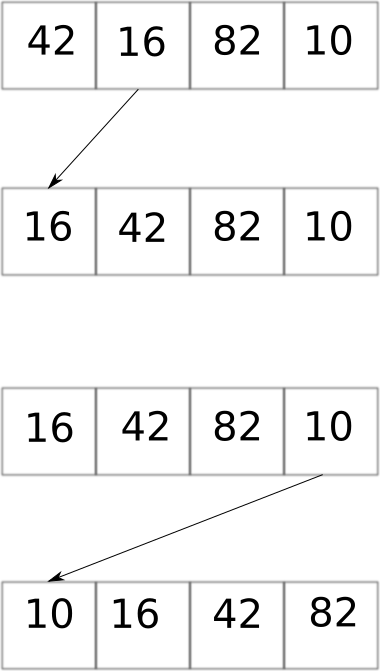
\includegraphics[width=0.3\linewidth]{figures/diagrams/sort/serialsort}
		\end{figure}	
\end{frame}

\begin{frame}
		\frametitle{Parallel Sort}
		\begin{figure}
				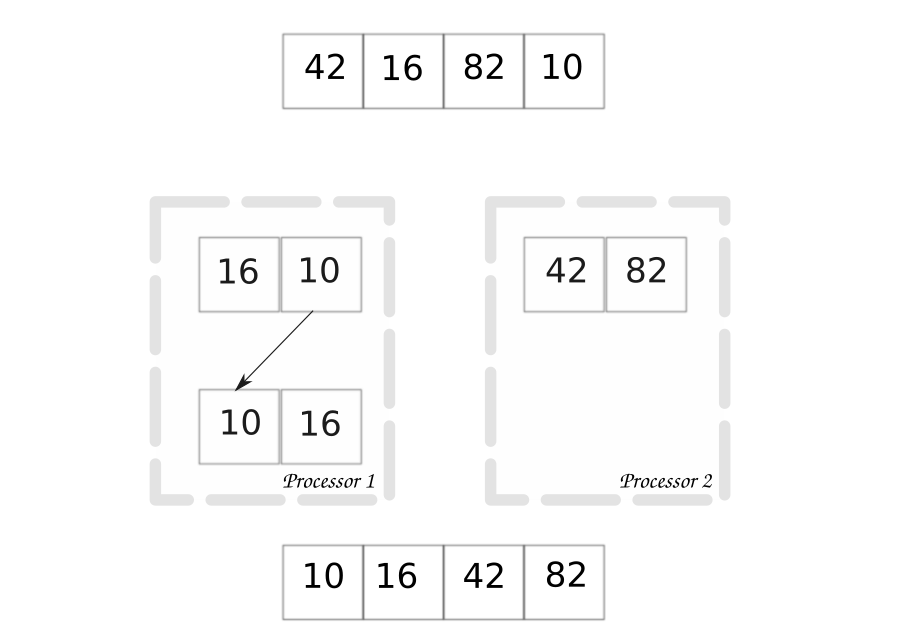
\includegraphics[width=0.8\linewidth]{figures/diagrams/sort/parallelsort}
		\end{figure}	
\end{frame}

\begin{frame}
		\frametitle{Observed Speedup}
		\begin{figure}
				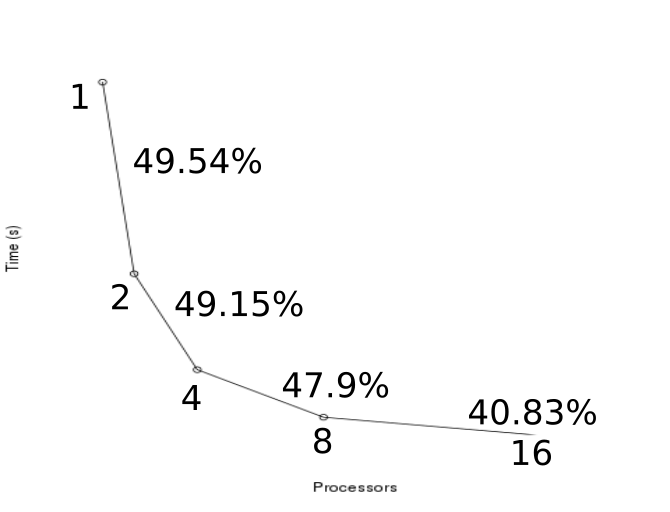
\includegraphics[width=0.7\linewidth]{figures/diagrams/omp/reduction}
		\end{figure}
\end{frame}

\begin{frame}
		\frametitle{Observed Speedup}
		\Huge{12.64x}
\end{frame}


\begin{frame}
		\frametitle{Amdahl's law}
		\begin{figure}
				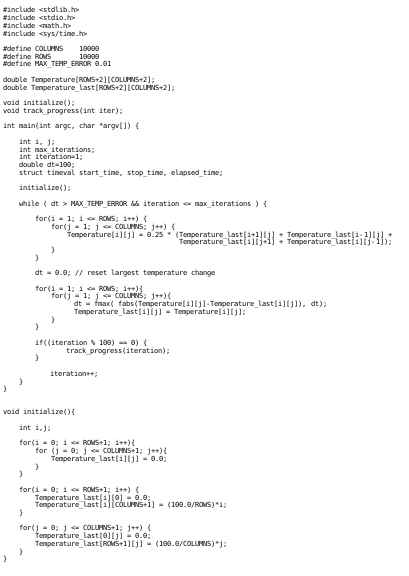
\includegraphics[width=0.4\linewidth]{figures/diagrams/amdahl/code}
		\end{figure}
\end{frame}

\begin{frame}
		\frametitle{Amdahl's law}
		\begin{figure}
				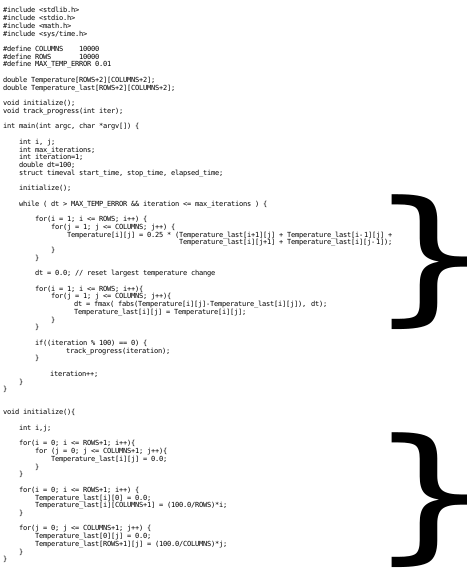
\includegraphics[width=0.4\linewidth]{figures/diagrams/amdahl/parallelblocks}
		\end{figure}
\end{frame}

\begin{frame}
		\frametitle{Amdahl's law}
		72 total lines of code 

		24 parallelizable lines of code
\end{frame}

\begin{frame}
		\frametitle{Parallel Overhead}
		\begin{figure}
				\includegraphics[width=0.4\linewidth]{figures/diagrams/amdahl/overhead}
		\end{figure}
\end{frame}
